% Options for packages loaded elsewhere
% Options for packages loaded elsewhere
\PassOptionsToPackage{unicode}{hyperref}
\PassOptionsToPackage{hyphens}{url}
\PassOptionsToPackage{dvipsnames,svgnames,x11names}{xcolor}
%
\documentclass[
]{article}
\usepackage{xcolor}
\usepackage[top=10pc,bottom=10pc,left=11pc,right=11pc,heightrounded]{geometry}
\usepackage{amsmath,amssymb}
\setcounter{secnumdepth}{-\maxdimen} % remove section numbering
\usepackage{iftex}
\ifPDFTeX
  \usepackage[T1]{fontenc}
  \usepackage[utf8]{inputenc}
  \usepackage{textcomp} % provide euro and other symbols
\else % if luatex or xetex
  \usepackage{unicode-math} % this also loads fontspec
  \defaultfontfeatures{Scale=MatchLowercase}
  \defaultfontfeatures[\rmfamily]{Ligatures=TeX,Scale=1}
\fi
\usepackage{lmodern}
\ifPDFTeX\else
  % xetex/luatex font selection
  \setmainfont[Numbers=Proportional,Numbers=OldStyle]{Linux Libertine O}
\fi
% Use upquote if available, for straight quotes in verbatim environments
\IfFileExists{upquote.sty}{\usepackage{upquote}}{}
\IfFileExists{microtype.sty}{% use microtype if available
  \usepackage[]{microtype}
  \UseMicrotypeSet[protrusion]{basicmath} % disable protrusion for tt fonts
}{}


\usepackage{longtable,booktabs,array}
\usepackage{calc} % for calculating minipage widths
% Correct order of tables after \paragraph or \subparagraph
\usepackage{etoolbox}
\makeatletter
\patchcmd\longtable{\par}{\if@noskipsec\mbox{}\fi\par}{}{}
\makeatother
% Allow footnotes in longtable head/foot
\IfFileExists{footnotehyper.sty}{\usepackage{footnotehyper}}{\usepackage{footnote}}
\makesavenoteenv{longtable}
\usepackage{graphicx}
\makeatletter
\newsavebox\pandoc@box
\newcommand*\pandocbounded[1]{% scales image to fit in text height/width
  \sbox\pandoc@box{#1}%
  \Gscale@div\@tempa{\textheight}{\dimexpr\ht\pandoc@box+\dp\pandoc@box\relax}%
  \Gscale@div\@tempb{\linewidth}{\wd\pandoc@box}%
  \ifdim\@tempb\p@<\@tempa\p@\let\@tempa\@tempb\fi% select the smaller of both
  \ifdim\@tempa\p@<\p@\scalebox{\@tempa}{\usebox\pandoc@box}%
  \else\usebox{\pandoc@box}%
  \fi%
}
% Set default figure placement to htbp
\def\fps@figure{htbp}
\makeatother


% definitions for citeproc citations
\NewDocumentCommand\citeproctext{}{}
\NewDocumentCommand\citeproc{mm}{%
  \begingroup\def\citeproctext{#2}\cite{#1}\endgroup}
\makeatletter
 % allow citations to break across lines
 \let\@cite@ofmt\@firstofone
 % avoid brackets around text for \cite:
 \def\@biblabel#1{}
 \def\@cite#1#2{{#1\if@tempswa , #2\fi}}
\makeatother
\newlength{\cslhangindent}
\setlength{\cslhangindent}{1.5em}
\newlength{\csllabelwidth}
\setlength{\csllabelwidth}{3em}
\newenvironment{CSLReferences}[2] % #1 hanging-indent, #2 entry-spacing
 {\begin{list}{}{%
  \setlength{\itemindent}{0pt}
  \setlength{\leftmargin}{0pt}
  \setlength{\parsep}{0pt}
  % turn on hanging indent if param 1 is 1
  \ifodd #1
   \setlength{\leftmargin}{\cslhangindent}
   \setlength{\itemindent}{-1\cslhangindent}
  \fi
  % set entry spacing
  \setlength{\itemsep}{#2\baselineskip}}}
 {\end{list}}
\usepackage{calc}
\newcommand{\CSLBlock}[1]{\hfill\break\parbox[t]{\linewidth}{\strut\ignorespaces#1\strut}}
\newcommand{\CSLLeftMargin}[1]{\parbox[t]{\csllabelwidth}{\strut#1\strut}}
\newcommand{\CSLRightInline}[1]{\parbox[t]{\linewidth - \csllabelwidth}{\strut#1\strut}}
\newcommand{\CSLIndent}[1]{\hspace{\cslhangindent}#1}



\setlength{\emergencystretch}{3em} % prevent overfull lines

\providecommand{\tightlist}{%
  \setlength{\itemsep}{0pt}\setlength{\parskip}{0pt}}





% -----------------------
% CUSTOM PREAMBLE STUFF
% -----------------------

% -----------------
% Typography tweaks
% -----------------
% Sets the paragraph indent size. 1pc is a pica (12pt). 
% This controls how much the first line of a paragraph is indented.
\setlength{\parindent}{1pc}

% The nowidow package tries to prevent widows and orphans 
% (single lines of a paragraph stranded at top/bottom of a page). 
% defaultlines=2 requests at least two lines to remain on a page when possible.
\usepackage[all,defaultlines=2]{nowidow}

% enumitem gives fine control of lists.

  % \setlist[1]{labelindent=\parindent}: for first-level lists, 
  % set the label indent equal to the paragraph indent 
  % (keeps list labels aligned with normal text).
  % 
  % leftmargin=* on itemize/enumerate: tells enumitem to align the 
  % list body with the surrounding text (remove extra left offset).

\usepackage{enumitem}
\setlist[1]{labelindent=\parindent}
\setlist[itemize]{leftmargin=*}
\setlist[enumerate]{leftmargin=*}

 % description with style=unboxed makes description-list terms wrap 
% nicely (no boxed layout).
\setlist[description]{style=unboxed}


% Improves Table of Contents formatting (the titles option makes it 
% play nicely with section title formatting).
\usepackage[titles]{tocloft}

% Remove left margin in lists inside longtables
% https://tex.stackexchange.com/a/378190/11851
\AtBeginEnvironment{longtable}{\setlist[itemize]{nosep, wide=0pt, leftmargin=*, before=\vspace*{-\baselineskip}, after=\vspace*{-\baselineskip}}}

% Allow for /singlespacing and /doublespacing
\usepackage{setspace}


% -----------------
% Title block stuff
% -----------------

% Abstract
\usepackage[overload]{textcase}
\usepackage[runin]{abstract}
\renewcommand{\abstractnamefont}{\sffamily\footnotesize\bfseries\MakeUppercase}
\renewcommand{\abstracttextfont}{\sffamily\small}
\setlength{\absleftindent}{\parindent * 2}
\setlength{\absrightindent}{\parindent * 2}
\abslabeldelim{\quad}
\setlength{\abstitleskip}{-\parindent}


% Keywords
\newenvironment{keywords}
{\vskip -3em \hspace{\parindent}\small\sffamily{\sffamily\footnotesize\bfseries\MakeUppercase{Keywords}}\quad}
{\vskip 3em}

  
% Title
\usepackage{titling}
\setlength{\droptitle}{3em}
\pretitle{\par\vskip 5em \begin{flushleft}\LARGE\sffamily\bfseries}
\posttitle{\par\end{flushleft}\vskip 0.75em}


% Authors
%
% PHEW this is complicated for a number of reasons!
%
% When using \and with multiple authors, the article class in LaTeX wraps each 
% author block in a tabluar environment with a hardcoded center alignment. It's 
% possible to use \preauthor{} to start tabulars with a left alignment {l}, but 
% that only applies to the first author because the others all use \and with the 
% hardcoded {c}. But we can override the \and command and add our own {l}
%
% (See https://github.com/rstudio/rmarkdown/issues/1716#issuecomment-560601691 
% for an example of redefining \and to just be \\)
%
% That's all great, except tabulars have some amount of default horizontal 
% padding, which makes left-aligned author blocks not actuall get fully 
% left-aligned on the page. We can set the horizontal padding for the column to 
% 0, but it requires some wonky syntax: {@{\hspace{0em}}l@{}}
\renewcommand{\and}{\end{tabular} \hskip 3em \begin{tabular}[t]{@{\hspace{0em}}l@{}}}
\preauthor{\begin{flushleft}
           \lineskip 1.5em 
           \begin{tabular}[t]{@{\hspace{0em}}l@{}}}
\postauthor{\end{tabular}\par\end{flushleft}}

% Omit the date since the \published command does that
\predate{}
\postdate{}

% Command for a note at the top of the first page describing the publication
% status of the paper.
\newcommand{\published}[1]{%
   \gdef\puB{#1}}
   \newcommand{\puB}{}
   \renewcommand{\maketitlehooka}{%
       \par\noindent\footnotesize\sffamily \puB}


% ------------------
% Section headings
% ------------------
\usepackage{titlesec}
\titleformat*{\section}{\Large\sffamily\bfseries\raggedright}
\titleformat*{\subsection}{\large\sffamily\bfseries\raggedright}
\titleformat*{\subsubsection}{\normalsize\sffamily\bfseries\raggedright}
\titleformat*{\paragraph}{\small\sffamily\bfseries\raggedright}

% \titlespacing{<command>}{<left>}{<before-sep>}{<after-sep>}
% Starred version removes indentation in following paragraph
\titlespacing*{\section}{0em}{2em}{0.1em}
\titlespacing*{\subsection}{0em}{1.25em}{0.1em}
\titlespacing*{\subsubsection}{0em}{0.75em}{0em}


% -----------
% Footnotes
% -----------
% NB: footmisc has to come after setspace and biblatex because of conflicts
\usepackage[bottom, flushmargin]{footmisc}
\renewcommand*{\footnotelayout}{\footnotesize}

\addtolength{\skip\footins}{10pt}    % vertical space between rule and main text
\setlength{\footnotesep}{5pt}  % vertical space between footnotes


% ----------
% Captions
% ----------
\usepackage[font={small,sf}, labelfont={small,sf,bf}]{caption}


% --------
% Macros
% --------
% pandoc will not convert text within \begin{} XXX \end{} to Markdown and will
% treat it as regular TeX. Because of this, it's impossible to do stuff like
% this:

% \begin{landscape}
%
% | One | Two   |
% |-----+-------|
% | my  | table |
% | is  | nice  |
%
% \end{landscape}
%
% Since it'll render like: | One | Two | |—–+——-| | my | table | | is | nice |
% 
% BUT, from this http://stackoverflow.com/a/41945462/120898 we can get around
% this by creating new commands for \begin and \end, like this:
\usepackage{pdflscape}
\newcommand{\blandscape}{\begin{landscape}}
\newcommand{\elandscape}{\end{landscape}}

% \blandscape
%
% | One | Two   |
% |-----+-------|
% | my  | table |
% | is  | nice  |
%
% \elandscape

% Same thing, but for generic groups
% But can't use \bgroup and \egroup because those are built-in TeX things
\newcommand{\stgroup}{\begingroup}
\newcommand{\fingroup}{\endgroup}


% ---------------------------
% END CUSTOM PREAMBLE STUFF
% ---------------------------
\usepackage{float}
\usepackage{tabularray}
\usepackage[normalem]{ulem}
\usepackage{graphicx}
\usepackage{rotating}
\UseTblrLibrary{siunitx}
\NewTableCommand{\tinytableDefineColor}[3]{\definecolor{#1}{#2}{#3}}
\newcommand{\tinytableTabularrayUnderline}[1]{\underline{#1}}
\newcommand{\tinytableTabularrayStrikeout}[1]{\sout{#1}}
\usepackage{mathtools}
\everydisplay\expandafter{\the\everydisplay\small }

\SetTblrStyle{foot}{font=\footnotesize}
\makeatletter
\@ifpackageloaded{caption}{}{\usepackage{caption}}
\AtBeginDocument{%
\ifdefined\contentsname
  \renewcommand*\contentsname{Table of contents}
\else
  \newcommand\contentsname{Table of contents}
\fi
\ifdefined\listfigurename
  \renewcommand*\listfigurename{List of Figures}
\else
  \newcommand\listfigurename{List of Figures}
\fi
\ifdefined\listtablename
  \renewcommand*\listtablename{List of Tables}
\else
  \newcommand\listtablename{List of Tables}
\fi
\ifdefined\figurename
  \renewcommand*\figurename{Figure}
\else
  \newcommand\figurename{Figure}
\fi
\ifdefined\tablename
  \renewcommand*\tablename{Table}
\else
  \newcommand\tablename{Table}
\fi
}
\@ifpackageloaded{float}{}{\usepackage{float}}
\floatstyle{ruled}
\@ifundefined{c@chapter}{\newfloat{codelisting}{h}{lop}}{\newfloat{codelisting}{h}{lop}[chapter]}
\floatname{codelisting}{Listing}
\newcommand*\listoflistings{\listof{codelisting}{List of Listings}}
\makeatother
\makeatletter
\makeatother
\makeatletter
\@ifpackageloaded{caption}{}{\usepackage{caption}}
\@ifpackageloaded{subcaption}{}{\usepackage{subcaption}}
\makeatother
\usepackage{bookmark}
\IfFileExists{xurl.sty}{\usepackage{xurl}}{} % add URL line breaks if available
\urlstyle{same}
\hypersetup{
  pdftitle={Procrastination as a Marker of Cognitive Decline: Evidence from Longitudinal Transitions in the Older Adult Population},
  pdfauthor={Cormac Monaghan; Rafael de Andrade Moral; Michelle Kelly; Joanna McHugh Power},
  pdfkeywords={Dementia risk, Mild cognitive
impairment, Procrastination, Apathy, Executive dysfunction, Aging;},
  colorlinks=true,
  linkcolor={DarkSlateBlue},
  filecolor={Maroon},
  citecolor={DarkSlateBlue},
  urlcolor={DarkSlateBlue},
  pdfcreator={LaTeX via pandoc}}


% -----------------------
% END-OF-PREAMBLE STUFF
% -----------------------


% ---------------------- 
% Title block elements
% ---------------------- 
\usepackage{orcidlink}  % Create automatic ORCID icons/links

\title{Procrastination as a Marker of Cognitive Decline: Evidence from
Longitudinal Transitions in the Older Adult Population}


\author{
{\large Cormac Monaghan~\orcidlink{0000-0001-9012-3060}}%
\thanks{Corresponding author.} \\%
Maynooth University \\%
{\footnotesize \url{cormacmonaghan@protonmail.com}} \and
{\large Rafael de Andrade Moral~\orcidlink{0000-0002-0875-3563}}%
 \\%
Maynooth University \\%
{\footnotesize \url{}} \and
{\large Michelle Kelly~\orcidlink{0000-0001-6159-6707}}%
 \\%
National College of Ireland \\%
{\footnotesize \url{}} \and
{\large Joanna McHugh Power~\orcidlink{0000-0002-7387-3107}}%
 \\%
Maynooth University \\%
{\footnotesize \url{}} \and
}

\date{}


% Typeset URLs in the same font as their parent environment
%
% This has to come at the end of the preamble, after any biblatex stuff because 
% some biblatex styles (like APA) define their own \urlstyle{}
\usepackage{url}
\urlstyle{same}

% ---------------------------
% END END-OF-PREAMBLE STUFF
% ---------------------------
\begin{document}
% ---------------
% TITLE SECTION
% ---------------
\published{\textbf{} \\ {\scriptsize Access the code, data, and analysis
at \url{https://github.com/C-Monaghan/crisp-clam}}}

\maketitle

\begin{abstract}
Cognitive decline is a global health concern, making the identification
of early, modifiable risk factors essential. While apathy is a
recognized prodromal marker, procrastination may also signal early
executive dysfunction. We used longitudinal secondary data from the
United States Health and Retirement Study among adults aged 60+
\((n = 549; \bar{x} = 69.70;\sigma = 7.58)\). Cognitive function,
procrastination, and a proxy measure of apathy were assessed.
Transitions between normative cognitive function, mild cognitive
impairment (MCI), and dementia were modeled using a discrete-time
first-order Markov model. Procrastination scores were higher among
individuals with MCI or dementia than those with normative cognitive
function. Procrastination also interacted with age, disproportionately
increasing the risk of decline in the oldest participants.
Procrastination was associated with cognitive impairment and predicted
transitions to MCI, suggesting it may serve as both an early behavioral
marker and compounding risk factor.
\end{abstract}
\vskip 3em

\begin{keywords}
\def\sep{;\ }
Dementia risk\sep Mild cognitive
impairment\sep Procrastination\sep Apathy\sep Executive dysfunction\sep 
Aging;
\end{keywords}
% -------------------
% END TITLE SECTION
% -------------------

Dementia is characterized by progressive decline of cognitive function,
leading to memory loss and difficulties with daily living
(\citeproc{ref-prince2013}{Prince et al., 2013};
\citeproc{ref-sanz-blasco2022}{Sanz-Blasco et al., 2022}). The global
burden of dementia is substantial, with cases projected to rise to 152.8
million by 2050 (\citeproc{ref-nichols2022}{Nichols et al., 2022}).
Identifying and addressing modifiable risk factors is crucial to
mitigate this projected rise in prevalence. Two particularly vulnerable
groups are older adults and those with mild cognitive impairment (MCI),
of whom up to 80\% progress to dementia within six years Tschanz et al.
(\citeproc{ref-tschanz2006}{2006}).

The Lancet Commission on Dementia identified fourteen causal risk
factors including smoking, hypertension, and diabetes, which account for
approximately 45\% of dementia cases worldwide
(\citeproc{ref-livingston2024}{Livingston et al., 2024}). Prodromal
markers, on the other hand, reflect early disease processes and may
signal limited opportunities for prevention
(\citeproc{ref-teipel2025}{Teipel et al., 2025}). One such prodromal
marker is apathy, or the significant loss of motivation, as distinct
from depression and cognitive impairment
(\citeproc{ref-fresnais2023}{Fresnais et al., 2023};
\citeproc{ref-richard2012}{Richard et al., 2012}). Apathy is prevalent
in both MCI and dementia subgroups Salem et al.
(\citeproc{ref-salem2023}{2023}). Apathy is a significant predictor of
the transition from MCI to dementia van Dalen et al.
(\citeproc{ref-vandalen2018}{2018}). While apathy has been
well-established as a prodromal marker and risk factor for dementia
progression, emerging evidence suggests that procrastination may also
relate to early cognitive decline.

Though superficially similar, apathy and procrastination are
behaviorally distinct. Apathy reflects reduced internal drive and
emotional engagement, impairing initiation of action
(\citeproc{ref-fresnais2023}{Fresnais et al., 2023}), whereas
procrastination reflects intact intention but delayed execution
(\citeproc{ref-steel2007}{Steel, 2007}). While both reflect impairments
in executive functioning, procrastination may additionally capture
unique aspects of emotional and motivational dysregulation . For
instance, person A may feel no motivation to attend an exercise class
and therefore never books it (apathy). Person B, however, books the
class and intends to go, but postpones at the last minute
(procrastination). Both apathy and procrastination have been linked to
dysfunction in prefrontal regions implicated in dementia
(\citeproc{ref-fahed2021}{Fahed \& Steffens, 2021};
\citeproc{ref-friden2020}{Fridén, 2020};
\citeproc{ref-joseph2021}{Joseph et al., 2021};
\citeproc{ref-zhang2010}{Y. F. Zhang et al., 2010}).

These parallels raise the possibility that procrastination could serve
as an early marker of cognitive impairment or even a modifiable risk
factor. Chronic procrastination may exacerbate decline by limiting
engagement in cognitively stimulating activities such as physical
exercise, problem-solving, and goal-setting, which build cognitive
resilience and reduce dementia risk
(\citeproc{ref-chowdhary2022}{Chowdhary et al., 2022};
\citeproc{ref-kelly2021}{Kelly \& Walton, 2021};
\citeproc{ref-livingston2024}{Livingston et al., 2024};
\citeproc{ref-mohammadibytamar2020}{Mohammadi Bytamar et al., 2020}).
Reduced engagement may contribute to a cycle of cognitive disengagement,
accelerating decline.

Importantly, procrastination is responsive to intervention through
cognitive-behavioral strategies and self-regulation training
(\citeproc{ref-rozental2014}{Rozental \& Carlbring, 2014};
\citeproc{ref-vaneerde2018}{van Eerde \& Klingsieck, 2018}). Crucially,
procrastination may identify individuals with motivational or executive
dysfunction who do not yet meet the long-term symptom threshold for
apathy, offering a potentially valuable and earlier marker (and possible
target) for neurodegenerative risk.

Since age remains the strongest predictor of MCI and dementia, it is
important to consider how procrastination operates across the lifespan
(i.e.~interaction with age). Many established modifiable risk factors
such as hypertension, hearing loss, smoking, and social isolation, exert
age-dependent effects, with certain factors carrying more weight at
midlife than in late life (\citeproc{ref-livingston2020}{Livingston et
al., 2020}, \citeproc{ref-livingston2024}{2024}). Understanding how
procrastination interacts with age may help clarify its role in the
aetiology of cognitive decline and identify windows of opportunity for
targeted intervention.

To our knowledge, no studies have directly examined procrastination as a
predictor of cognitive decline or dementia progression. Accordingly, the
present study aimed to a) assess differences in procrastination levels
across three groups: individuals with dementia, individuals with MCI,
and individuals with neither dementia nor MCI, and b) test whether
higher procrastination scores predict transition from normative
cognition function to dementia or MCI to dementia.

\section{Method}\label{method}

\subsection{Data and study population}\label{data-and-study-population}

Analyses were conducted using a secondary data source; a multi-wave
prospective cohort study called the Health and Retirement Study (HRS;
(\citeproc{ref-fisher2018}{Fisher \& Ryan, 2018}), which tracks the
health, economic, and social well-being of over \(18,000\) American
adults primarily aged \(50+\). The HRS is managed by the Institute for
Social Research at the University of Michigan, with data collected every
two years. Initial data collection of a participant is conducted through
a face-to-face interview, with follow-up biennial interviews conducted
either by phone or face-to-face. The average retention rate ranges from
\(68.8\%\) to \(92.3\%\) (\citeproc{ref-HRS2017}{Health and Retirement
Study, 2017}). At the time of writing, fifteen years of HRS data are
currently archived.

We focused on four waves of HRS data from 2016 to 2022. Specifically,
our study sample consisted of respondents who participated in an
experimental module assessing procrastination during the 2020 wave.
These experimental modules, administered at the end of the core HRS
interview, consist of concise questionnaires designed to explore new
topics or supplement existing core survey data
(\citeproc{ref-juster1995}{Juster \& Suzman, 1995}). Each respondent
receives only one experimental module, with sample sizes for each module
constituting approximately 10\% of the core sample. As a result, while
the core HRS sample includes approximately \(18,000\) respondents, our
initial sample of interest consisted of \(1,368\) respondents. We
excluded respondents with missing cognitive assessment data for any wave
\((n = 419)\), those under 60 years of age, (as cognitive symptoms
typically occur around this age \(n = 398\)), and those with complete
missing values across the procrastination measure \((n = 2)\). This
resulted in a final analytic sample of \(549\) respondents.

\subsection{Measures}\label{measures}

\subsubsection{Outcome: Cognitive Function and Cognitive
Category}\label{outcome-cognitive-function-and-cognitive-category}

Cognitive function in the HRS is assessed using a series of tests
adapted from the Telephone Interview for Cognitive Status (TICS;
(\citeproc{ref-brandt1988}{Brandt et al., 1988};
\citeproc{ref-fong2009}{Fong et al., 2009}). These tests include an
immediate and delayed \(10\)-noun free recall test (to assess episodic
memory), a serial seven subtraction test (to assess working memory), and
a backward count from \(20\) test (to assess mental processing). Based
on these assessments, Crimmins et al.
(\citeproc{ref-crimmins2011}{2011}) developed both a \(27\)-point
cognitive scale and validated cut-off points to assess and classify
cognitive status. Using these points, respondents who scored \(12 - 27\)
were classified as having normal cognition, \(7 - 11\) as having MCI,
and \(0 - 6\) as having dementia.

\subsubsection{Predictor:
Procrastination}\label{predictor-procrastination}

Procrastination was measured using the Pure Procrastination Scale
(\citeproc{ref-steel2010}{Steel, 2010}), a psychometrically validated
scale for evaluating procrastination when conceptualized as a
dysfunctional delay. The PPS consists of 12 items rated on a Likert
scale ranging from \(1\) (strongly disagree) to \(5\) (strongly agree).
In responding to the scale items, participants were asked to reflect on
their general behavioural tendencies, with no specific time-frame
provided. Total procrastination scores range from \(12\) to \(60\), with
higher scores indicating greater tendency to procrastinate. In the HRS,
the PPS was administered only in wave 3 (2020) of the respective waves.
As such, we use the wave 3 measure as both a retrospective and
prospective proxy for procrastination scores across all waves in the
analysis. This approach assumes relative temporal stability in
procrastination over the study period. In this sample, the PSS had a
Cronbach's \(\alpha\) score of 0.92, indicating high internal
consistency. In responding to the scale items, participants were asked
to reflect on their general behavioural tendencies, with no specific
time-frame provided. An example of a question from the scale includes
``I delay making decisions until it's too late''.

\subsubsection{Covariate: Apathy}\label{covariate-apathy}

While no direct measure of apathy exists within the HRS, we utilised two
questions from the eight-item version of the Center for Epidemiological
Studies Depression (CES-D8) scale (\citeproc{ref-briggs2018}{Briggs et
al., 2018}) as proxies for apathy: ``You felt that everything you did
was an effort'' and ``You could not get going''. Both items capture core
features of apathy (behavioural and motivational disengagement) and,
while not a comprehensive measure of apathy, provide a valid and
pragmatic approximation for modelling purposes. Each item was measured
on a binary ``yes/no'' scale with total scores ranging from \$0\$ to
\$2\$.

\subsubsection{Confounders}\label{confounders}

To account for potential confounding, we controlled for demographic
variables with established associations with both cognitive function and
procrastination (\citeproc{ref-vanderweele2019}{VanderWeele, 2019}).
These included measures of age, sex, and educational attainment
(\citeproc{ref-abner2012}{Abner et al., 2012};
\citeproc{ref-freedman2024}{Freedman \& Cornman, 2024};
\citeproc{ref-yu2013}{Yu et al., 2013}). Educational attainment was
classified into three categories: no formal education, GED (General
Educational Development)/high school diploma, and college/further
education.

\clearpage

\subsection{Data Analysis}\label{data-analysis}

All data analysis was carried out in R (\citeproc{ref-rcoreteam2025}{R
Core Team, 2025}). To model transitions in cognitive states over time,
we employed a first order discrete-time Markov model, a class of
stochastic processes that satisfy the Markov property
(\citeproc{ref-zhang2010}{Y. F. Zhang et al., 2010}), which can be
formally expressed as:

\[P(X_{t+1} = j \vert X_t = i, X_{t-1} = i_{t-1}, \dots X_0 = i_0) = P(X_{t+1} = j \vert X_t = i)\]

This property asserts that the probability of transitioning from state
\$X\_t = i\$ to a future state \$X\_\{t+1\} = j\$ depends only on the
current state \$X\_t\$, and not on the full history of preceding states.
Here, there are three potential states: normative cognitive function,
mild cognitive impairment, and dementia. We consider dementia to be an
absorbing state, i.e.~once an individual reaches this state, they cannot
return to the other states in a future time point.

Unlike continuous-time models, discrete-time Markov models are not
readily supported by a dedicated R package for deriving transition
probabilities. Therefore, we implemented the model manually using
multinomial logistic regression from the \emph{nnet} package
(\citeproc{ref-venables2002}{Venables \& Ripley, 2002}). This approach
estimates the log-odds of transitioning to each non-reference state as a
linear function of covariates, relative to a chosen reference category.
For a system with \(K\) cognitive states (with state \(K\) as the
reference), the model takes the form:

\[log \frac{P(Y = j \; \vert \; x)}{P(Y = K \vert x)} = \beta_0 + \beta_j^\top x \qquad \text{for } j = 1, \dots K-1\]

From these equations, the predicted transition probabilities for the
non-reference states \(j = 1, \dots, K - 1\) are derived as:

\[P(Y = j \vert x) = \frac{e^{\beta_{0j} + \beta_j^\top x}}{1 + \sum^{K - 1}_{k = 1} e^{\beta_{0k} + \beta_k^ \top x}}\]

and for the reference state \(K\) as:

\[ P(Y = K \; \vert \; x) = \frac{1}{1 + \sum^{K - 1}_{k = 1} e^{\beta_{0k} + \beta_j^ \top x }} \]

To assess model fit and guide model selection for covariates in the
\(\beta_j\) vectors, we conducted likelihood-ratio tests comparing full
and reduced models, whose test statistic is defined as:

\[ D = 2 \times (\ell_{\text{reduced}} - \ell_{\text{full}}) \]

where \(\ell_{\text{full}}\) and \(\ell_{\text{reduced}}\) denote the
log-likelihoods of the respective models. Under the null hypothesis that
the full model does not represent an improved fit when compared to the
reduced model, \(D\) has an asymptotic \(\chi^2\) distribution with
degrees of freedom corresponding to the difference between the numbers
of parameters estimated by the two models.

\section{Results}\label{results}

Our final analytic sample comprised \(549\) respondents with the
following age distribution: 60 - 70 \((n = 186)\), 71 - 80
\((n = 203)\), 81 - 90 \((n = 142)\), and 90+ \((n = 18)\). Descriptive
statistics for the full sample, as well as data stratified by cognitive
status (normative cognitive function, MCI, and dementia), are presented
in Table~\ref{tbl-descriptives}. Both Figure~\ref{fig-river} and
supplementary figure S1 capture the unconditional transitions and
transition probabilities (respectively) between wave one and two (first
transition), wave two and three (second transition), and wave three and
four (third transition), yielding a total of \(1,647\) observed
transitions over time.

\begin{table}[H]

\caption{\label{tbl-descriptives}Baseline descriptives for the study
sample and stratified by cognitive status category.}

\centering{

\centering
\begin{talltblr}[         %% tabularray outer open
entry=none,label=none,
note{}={\emph{Note:} Descriptives for continuous and categorical variables are represented
using means ± standard deviations and percentages and frequencies respectively.
NC = Normative cognitive function; MCI = Mild cognitive impairment;
GED = General Educational Development.},
note{a}={Procrastination scores were collected in 2020 (Wave 3) and are presented
here for descriptive comparison, although they were not measured at
baseline.},
]                     %% tabularray outer close
{                     %% tabularray inner open
colspec={Q[]Q[]Q[]Q[]Q[]},
hline{2}={1-5}{solid, black, 0.05em},
hline{1}={1-5}{solid, black, 0.1em},
hline{12}={1-5}{solid, black, 0.1em},
cell{1-2,4-5,7-11}{2}={}{halign=c},
cell{1-2,4-5,7-11}{3}={}{halign=c},
cell{1-2,4-5,7-11}{4}={}{halign=c},
cell{1-2,4-5,7-11}{5}={}{halign=c},
cell{3,6}{1}={c=5}{halign=l},
cell{3,6}{2}={}{halign=l},
cell{3,6}{3}={}{halign=l},
cell{3,6}{4}={}{halign=l},
cell{3,6}{5}={}{halign=l},
}                     %% tabularray inner close
& Full sample (n = 549) & NC (n = 452) & MCI (n = 86) & Dementia (n = 11) \\
Age (years) & 69.70 ± 7.58 & 69.70 ± 7.55 & 69.60 ± 7.55 & 70.00 ± 9.89 \\
\textbf{Sex} & **Sex** & **Sex** & **Sex** & **Sex** \\
Male & 38.43\% (n = 211) & 39.82\% (n =180) & 32.56\% (n = 28) & 27.27\% (n = 3) \\
Female & 61.57\% (n = 338) & 60.18\% (n = 272) & 67.44\% (n = 58) & 72.73\% (n = 8) \\
\textbf{Education} & **Education** & **Education** & **Education** & **Education** \\
No degree & 16.24\% (n = 98) & 10.56\% (n = 47) & 39.53\% (n = 34) & 63.54\% (n = 7) \\
GED & 51.58\% (n = 279) & 51.91\% (n = 231) & 52.33\% (n = 45) & 27.27\% (n = 3) \\
Further education & 32.29\% (n = 175) & 37.53\% (n = 167) & 8.14\% (n = 7) & 9.09\% (n = 1) \\
Apathy & 0.37 ± 0.63 & 0.31 ± 0.59 & 0.65 ± 0.76 & 0.36 ± 0.51 \\
Procrastination\textsuperscript{a} & 28.60 ± 12.00 & 27.70 ± 11.30 & 32.10 ± 13.80 & 39.00 ± 16.00 \\
\end{talltblr}

}

\end{table}%

\begin{figure}[H]

\centering{

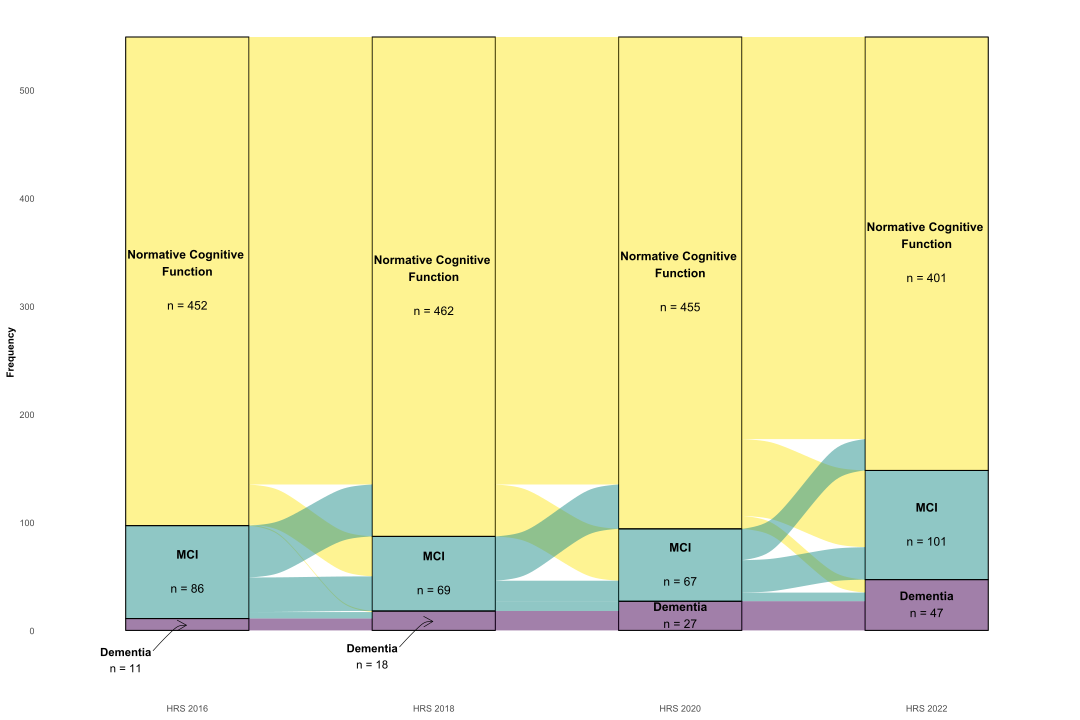
\includegraphics[width=1\linewidth,height=\textheight,keepaspectratio]{manuscript_files/figure-pdf/fig-river-1.pdf}

}

\caption{\label{fig-river}Frequency of cognitive status transitions
between HRS waves.}

\end{figure}%

\subsection{Cross sectional
differences}\label{cross-sectional-differences}

Initially, a Kruskal-Wallis test was conducted to examine differences in
procrastination scores (measured in 2020) across three cognitive status
groups after Levene's test indicated violation of homogeneity of
variance \((p = 0.039)\). The analysis revealed a statistically
significant effect of cognitive status,
\((\chi^2(2) = 17.54, p < .001)\), indicating that procrastination
levels differed significantly between at least two of the groups.
Post-hoc analysis using a pairwise Wilcoxon rank-sum test with a
Benjamini-Hochberg correction showed that participants with normal
cognition \((M = 27.7, SD = 11.7)\) reported significantly lower levels
of procrastination than those with both MCI
\((M = 32.1; SD = 11.3; p = 0.004)\) and dementia
\((M = 36.2; SD = 14.8; p = 0.005)\). No significance difference was
found between those with MCI and dementia \((p = 0.334)\).
Figure~\ref{fig-cross-sectional} displays the distribution of
procrastination scores across groups, with both boxplots and dotplots
showing median values and individual data points. Significance bars
indicate the pairwise differences described above.

\begin{figure}

\centering{

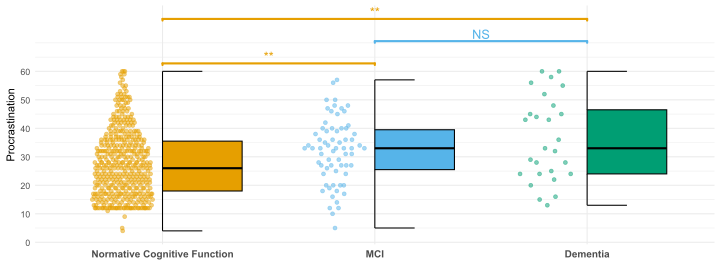
\includegraphics[width=1\linewidth,height=\textheight,keepaspectratio]{manuscript_files/figure-pdf/fig-cross-sectional-1.pdf}

}

\caption{\label{fig-cross-sectional}Group differences in 2020
procrastination scores according to cognitive status.}

\end{figure}%

\subsection{Markov analysis}\label{markov-analysis}

Results from the discrete-time Markov analysis, showed that all
covariates significantly influenced the likelihood of transitioning
between cognitive states (see Figure~\ref{fig-markov}). Notably,
procrastination interacted significantly with \emph{age} to affect two
key transitions: increasing the likelihood of transitioning from
normative cognitive function to MCI \((\text{OR} = 1.001; p < 0.001)\)
and decreasing the likelihood of reverting from MCI to normative
cognitive function \((\text{OR} = 0.999; p < 0.001)\). \emph{Women} were
significantly less likely than men to transition from both normative
cognitive function to dementia \((\text{OR} = 0.068; p < 0.001)\) and
from MCI to dementia \((\text{OR} = 0.70; p < 0.001\)).

For \emph{education attainment}, individuals with a GED were less likely
to transition from normative cognitive function to either MCI
\((\text{OR} = 0.49; p < 0.001)\) or dementia
\((\text{OR} = 0.29; p < 0.001)\) and from MCI to dementia
\((\text{OR} = 0.64; p < 0.001)\). They were also more likely to back
transition from MCI to normative cognitive function
\((\text{OR} = 2.18; p < 0.001)\). Those with a college level education
or higher demonstrated a significantly reduced likelihood of
transitioning from normative cognitive function to either MCI
\((\text{OR} = 0.32; p < 0.001)\) or dementia
\((\text{OR} = 0.07; p < 0.001)\) and from MCI to dementia
\((\text{OR} = 0.22; p < 0.001)\). They were also more likely to back
transition from MCI to normative cognitive function
\((\text{OR} = 3.13; p < 0.001)\).

Finally, higher levels of \emph{apathy} were associated with an
increased likelihood of transitioning from normative cognitive function
to both MCI \((\text{OR} = 1.35; p = 0.005)\) and dementia
\((\text{OR} = 1.36; p<0.001)\) and a decreased likelihood of
transitioning from MCI back to normative cognitive function
\((\text{OR} = 0.74; p = 0.003)\).

\begin{figure}

\centering{

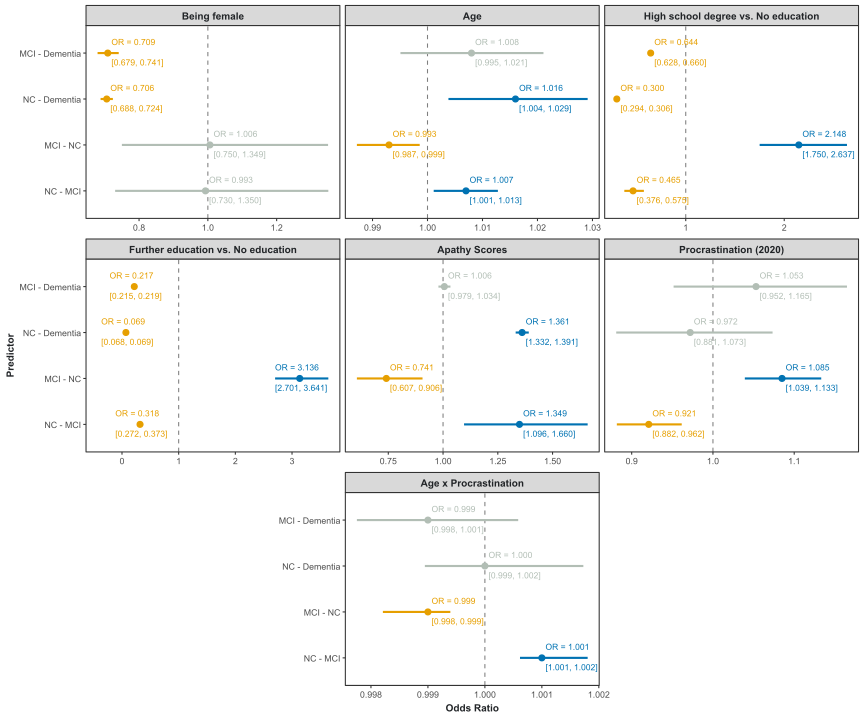
\includegraphics[width=1\linewidth,height=\textheight,keepaspectratio]{manuscript_files/figure-pdf/fig-markov-1.pdf}

}

\caption{\label{fig-markov}Odds ratios (95\% Confidence Intervals) of
transitioning from one cognitive state to another calculated using
generalised logit models. \emph{Note}. Odds ratios significantly
different from 1 at a 5\% significance rate are presented in blue
(positive) or orange (negative), otherwise they are presented in gray.
NC = Normative cognitive function; MCI = Mild cognitive impairment.}

\end{figure}%

Figure~\ref{fig-age-preds} presents the predicted transition
probabilities across varying levels of age and procrastination. These
estimates illustrate how the interaction between age and procrastination
influences the likelihood of progressing between cognitive states over
time. Notably, while transition probabilities remain relatively stable
at very low levels of procrastination, substantial shifts emerge as both
age and procrastination increase. In particular, older individuals with
higher procrastination scores show an elevated probability of cognitive
decline transitioning from normative cognitive function to mild
cognitive impairment (MCI) and a reduced likelihood of transitioning
back from MCI to normative cognitive function, highlighting the
compounded risk posed by these two variables in later life.

\begin{figure}

\centering{

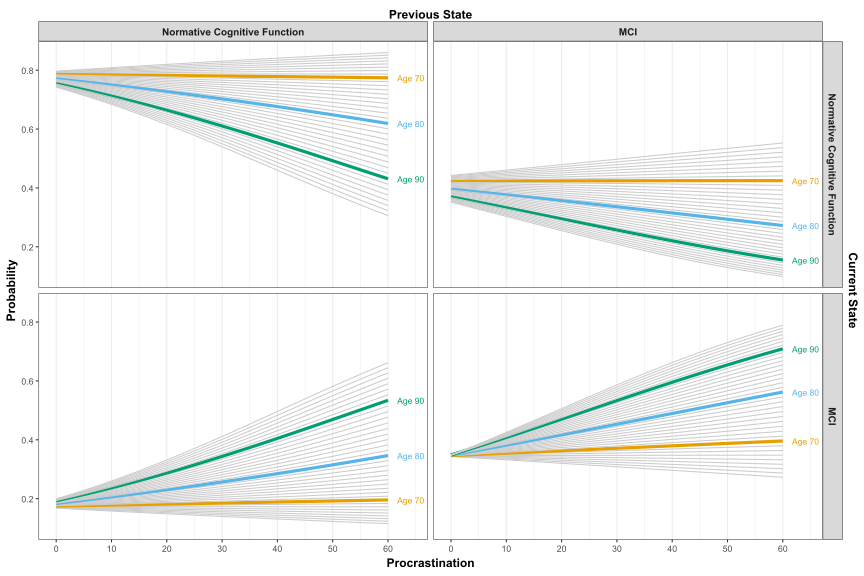
\includegraphics[width=1\linewidth,height=\textheight,keepaspectratio]{manuscript_files/figure-pdf/fig-age-preds-1.pdf}

}

\caption{\label{fig-age-preds}Predicted transition probabilities by
procrastination and age. \emph{Note.} Each curve represents a different
age profile, ranging from the minimum (62 years) to the maximum (97
years) of the dataset. Specific ages of interest (70, 80, and 90) are
highlighted.}

\end{figure}%

\section{Discussion}\label{discussion}

Dementia poses a growing global health burden, with modifiable risk
factors and prodromal markers offering important targets for
intervention (\citeproc{ref-livingston2020}{Livingston et al., 2020},
\citeproc{ref-livingston2024}{2024}). While apathy has been well
established as a prodromal marker and predictor of dementia
(\citeproc{ref-donovan2014}{Donovan et al., 2014};
\citeproc{ref-fresnais2023}{Fresnais et al., 2023};
\citeproc{ref-salem2023}{Salem et al., 2023};
\citeproc{ref-vandalen2018}{van Dalen et al., 2018}), emerging evidence
suggests that procrastination may also signal early cognitive
dysfunction (\citeproc{ref-friden2020}{Fridén, 2020};
\citeproc{ref-zhang2019}{S. Zhang et al., 2019}). This study examined
whether procrastination, particularly in later life, could serve as a
predictor of cognitive decline. We assessed both cross-sectional
differences in procrastination across three cognitive groups (normative
cognitive function, MCI and dementia) and longitudinal associations with
transitions in cognitive status, to clarify whether procrastination
functions as a novel and age-sensitive marker of emerging cognitive
impairment.

Our analysis revealed significant group differences in procrastination,
with individuals experiencing cognitive impairment, both MCI and
dementia, reporting higher procrastination scores than those with
normative cognitive function. These findings support the hypothesis that
procrastination may be associated with cognitive decline and aligns with
emerging evidence linking procrastination to cognitive dysfunction
(\citeproc{ref-friden2020}{Fridén, 2020}; \citeproc{ref-zhang2019}{S.
Zhang et al., 2019}). Interestingly, while both MCI and dementia groups
exhibited elevated procrastination scores, no significant difference
emerged between these two groups. This suggests that increases in
procrastination may occur relatively early in the neurodegenerative
process, potentially preceding or paralleling the emergence of more
overt cognitive symptoms.

However, it should be noted that the number of participants classified
as having MCI \((n = 67)\) or dementia \((n = 27)\) was relatively small
compared to those with normative cognitive function \((n = 455)\). This
imbalance in group sizes may have limited the sensitivity of our
comparisons and raises the possibility that subtle differences between
MCI and dementia groups were obscured by statistical power constraints.
Future research should aim to replicate these findings in more evenly
distributed samples to better determine whether procrastination
continues to increase across progressive stages of impairment or
plateaus following early decline.

Beyond these cross-sectional differences, our discrete-time Markov
analysis offered insight into how procrastination alongside other
demographic and psychological factors, influences the likelihood of
transitioning between cognitive states over time. Notably,
procrastination emerged as a dynamic predictor of cognitive change,
interacting with age to significantly increase the odds of transitioning
from normative cognitive function to MCI, while simultaneously
decreasing the odds of moving from MCI back to normative cognitive
function.

These findings imply that procrastination may serve dual roles, both as
a marker of early cognitive dysfunction and, potentially, as a
behavioral impediment to moving from MCI state to the normative
cognitive state. One plausible pathway involves the reinforcement of
maladaptive behaviors such as reduced cognitive engagement or reduced
participation in cognitively protective activities, such as physical
exercise, social interaction or medical adherence
(\citeproc{ref-hajek2025}{Hajek et al., 2025};
\citeproc{ref-kelly2021}{Kelly \& Walton, 2021};
\citeproc{ref-sirois2007}{Sirois, 2007}; \citeproc{ref-stead2010}{Stead
et al., 2010}). In parallel, procrastination has been associated with
chronic stress and elevated cortisol levels
(\citeproc{ref-sirois2023a}{Sirois, 2023}), which may accelerate
hippocampal atrophy, β-amyloid plaque deposition, and brain inflammation
(\citeproc{ref-franks2021}{Franks et al., 2021};
\citeproc{ref-wallensten2023}{Wallensten et al., 2023}), further
undermining cognitive resilience. These behavioral and biological
mechanisms align with self-regulation theories suggesting that
procrastination reflects executive dysfunction
(\citeproc{ref-rozental2014}{Rozental \& Carlbring, 2014};
\citeproc{ref-steel2007}{Steel, 2007}), an early feature of
neurodegenerative progression (\citeproc{ref-clark2012}{Clark et al.,
2012}).

The observed interaction with age (see Figure~\ref{fig-age-preds})
suggests that the influence of procrastination on cognitive trajectories
may grow stronger with advancing age, a period during which
neuro-plasticity diminishes, and behavioral risk factors exert greater
influence (\citeproc{ref-livingston2020}{Livingston et al., 2020},
\citeproc{ref-livingston2024}{2024}). This effect was particularly
pronounced among the oldest participants. As illustrated in
Figure~\ref{fig-age-preds}, the effect of procrastination is relatively
modest for younger-older adults (those age 70). However, the slope of
these transitions steepens considerably for individuals aged 80 and
especially for those age 90. These findings indicate that
procrastination is increasingly associated with a higher risk of
cognitive decline and a lower likelihood of improvement in cognitive
status in late old age.

This pattern underscores the possibility that procrastination functions
as a compounding risk factor in older adulthood, particularly among the
oldest individuals, by both reflecting emerging cognitive difficulties
and potentially accelerating their progression. In younger-old adults,
cognitive reserve and compensatory mechanisms
(\citeproc{ref-gooijers2024}{Gooijers et al., 2024}) may buffer against
the impact of poor self-regulation. However, as individuals reach more
advanced ages, these protective systems weaken
(\citeproc{ref-roberts2015}{Roberts et al., 2015}). Consequently,
maladaptive behavioral tendencies like procrastination can exert a
disproportionate toll on cognitive function. These findings underscore
the potential value of addressing behavioral regulation and
self-management in older adults as part of broader dementia
risk-reduction strategies, particularly for those of a much older age.

By revealing a significant interaction between age and procrastination,
this study highlights the importance of broadening dementia risk models
to incorporate dynamic lifestyle and psychological variables.
Procrastination, as both a modifiable and measurable behavioral tendency
(\citeproc{ref-vaneerde2018}{van Eerde \& Klingsieck, 2018}), represents
a promising target for low-cost, non-invasive interventions aimed at
enhancing cognitive resilience in older populations. Tracking
self-regulatory behavioral tendencies such as procrastination may offer
an early warning system for emerging cognitive risk, opening avenues for
preventative action before irreversible decline takes hold.

\subsection{Limitations}\label{limitations}

Despite the insights offered by this study, several limitations should
be considered. Most notably, although our longitudinal Markov modelling
approach captured changes in cognitive status, a key constraint was the
measurement of procrastination at only a single time point (2020). As a
result, we assumed temporal stability in procrastination scores across
time and used this measure as both a retrospective and prospective proxy
for procrastination scores. However, this precluded analysis of
within-person changes in this behavior over time and whether such
changes affect cognitive transitions. It should be noted that this
limitation is inherent to the HRS dataset rather than a methodological
oversight (Juster \& Suzman, 1995). Future studies should prioritise
repeated assessments of procrastination to determine whether increases
in procrastination precedes, accompanies, or follows cognitive decline.
Moreover, our use of a proxy measure of apathy may not have fully
captured the multidimensional nature of apathy. Future research should
incorporate more validated apathy assessments to strengthen the
behavioral inferences drawn.

Additionally, as noted earlier, the relatively small number of
individuals in the MCI and dementia groups may have constrained
statistical power for certain comparisons and increased the potential
for misclassification bias. Finally, while the models adjusted for
several key demographic and psychological covariates, unmeasured
confounding (undiagnosed medical conditions, medication use, or sleep
quality) could also have influenced cognitive outcomes. Future research
should seek to replicate and extend these findings using more clinically
diverse samples.

\subsection{Conclusions}\label{conclusions}

In summary, this study offers preliminary evidence that procrastination
may function as an early behavioral tendency marker of cognitive
decline, particularly in older age. Individuals with MCI and dementia
reported higher procrastination scores, and longitudinal modelling
revealed that procrastination, especially when coupled with advancing
age, was predictive of increased cognitive decline. These findings
underscore the importance of everyday self-regulatory behaviors in
dementia risk and resilience. As a modifiable and measurable construct,
procrastination holds promise as a target for early detection and
preventative intervention strategies aimed at sustaining cognitive
health in ageing populations.

\section*{References}\label{references}
\addcontentsline{toc}{section}{References}

\phantomsection\label{refs}
\begin{CSLReferences}{1}{0}
\bibitem[\citeproctext]{ref-abner2012}
Abner, E. L., Kryscio, R. J., Cooper, G. E., Fardo, D. W., Jicha, G. A.,
Mendiondo, M. S., Van Eldik, L. J., Wan, L., \& Schmitt, F. A. (2012).
Mild cognitive impairment: Statistical models of transition using
longitudinal clinical data. \emph{International Journal of Alzheimer's
Disease}, \emph{2012}(1), 291920.
\url{https://doi.org/10.1155/2012/291920}

\bibitem[\citeproctext]{ref-brandt1988}
Brandt, J., Spencer, M., \& Folstein, Marshal. (1988). The telephone
interview for cognitive status. \emph{Neuropsychiatry, Neuropsychology,
and Behavioral Neurology}, \emph{1}(2), 111--117.

\bibitem[\citeproctext]{ref-briggs2018}
Briggs, R., Carey, D., O'Halloran, A. M., Kenny, R. A., \& Kennelly, S.
P. (2018). Validation of the 8-item centre for epidemiological studies
depression scale in a cohort of community-dwelling older people: Data
from the irish longitudinal study on ageing ({TILDA}). \emph{European
Geriatric Medicine}, \emph{9}, 121--126.
\url{https://doi.org/10.1007/s41999-017-0016-0}

\bibitem[\citeproctext]{ref-chowdhary2022}
Chowdhary, N., Barbui, C., Anstey, K. J., Kivipelto, M., Barbera, M.,
Peters, R., Zheng, L., Kulmala, J., Stephen, R., Ferri, C. P., et al.
(2022). Reducing the risk of cognitive decline and dementia: {WHO}
recommendations. \emph{Frontiers in Neurology}, \emph{12}, 765584.
\url{https://doi.org/10.3389/fneur.2021.765584}

\bibitem[\citeproctext]{ref-clark2012}
Clark, L. R., Schiehser, D. M., Weissberger, G. H., Salmon, D. P.,
Delis, D. C., \& Bondi, M. W. (2012). Specific measures of executive
function predict cognitive decline in older adults. \emph{Journal of the
International Neuropsychological Society}, \emph{18}(1), 118--127.
\url{https://doi.org/10.1017/s1355617711001524}

\bibitem[\citeproctext]{ref-cooper2015}
Cooper, C., Sommerlad, A., Lyketsos, C. G., \& Livingston, G. (2015).
Modifiable predictors of dementia in mild cognitive impairment: A
systematic review and meta-analysis. \emph{American Journal of
Psychiatry}, \emph{172}(4), 323--334.
\url{https://doi.org/10.1176/appi.ajp.2014.14070878}

\bibitem[\citeproctext]{ref-crimmins2011}
Crimmins, E. M., Kim, J. K., Langa, K. M., \& Weir, D. R. (2011).
Assessment of cognition using surveys and neuropsychological assessment:
The health and retirement study and the aging, demographics, and memory
study. \emph{Journals of Gerontology Series B: Psychological Sciences
and Social Sciences}, \emph{66}, i162--i171.
\url{https://doi.org/10.1093/geronb/gbr048}

\bibitem[\citeproctext]{ref-donovan2014}
Donovan, N. J., Wadsworth, L. P., Lorius, N., Locascio, J. J., Rentz, D.
M., Johnson, K. A., Sperling, R. A., Marshall, G. A., Initiative, A. D.
N., et al. (2014). Regional cortical thinning predicts worsening apathy
and hallucinations across the {Alzheimer} disease spectrum. \emph{The
American Journal of Geriatric Psychiatry}, \emph{22}(11), 1168--1179.
\url{https://doi.org/10.1016/j.jagp.2013.03.006}

\bibitem[\citeproctext]{ref-fahed2021}
Fahed, M., \& Steffens, D. C. (2021). Apathy: Neurobiology, assessment
and treatment. \emph{Clinical Psychopharmacology and Neuroscience},
\emph{19}(2), 181. \url{https://doi.org/10.9758/cpn.2021.19.2.181}

\bibitem[\citeproctext]{ref-fisher2018}
Fisher, G. G., \& Ryan, L. H. (2018). Overview of the health and
retirement study and introduction to the special issue. \emph{Work,
Aging and Retirement}, \emph{4}(1), 1--9.
\url{https://doi.org/10.1093/workar/wax032}

\bibitem[\citeproctext]{ref-fong2009}
Fong, T. G., Fearing, M. A., Jones, R. N., Shi, P., Marcantonio, E. R.,
Rudolph, J. L., Yang, F. M., Kiely, D. K., \& Inouye, S. K. (2009).
Telephone interview for cognitive status: {Creating} a crosswalk with
the mini-mental state examination. \emph{Alzheimer's \& Dementia},
\emph{5}(6), 492--497. \url{https://doi.org/10.1016/j.jalz.2009.02.007}

\bibitem[\citeproctext]{ref-franks2021}
Franks, K. H., Bransby, L., Saling, M. M., \& Pase, M. P. (2021).
Association of stress with risk of dementia and mild cognitive
impairment: A systematic review and meta-analysis. \emph{Journal of
Alzheimer's Disease}, \emph{82}(4), 1573--1590.
\url{https://doi.org/10.3233/jad-210094}

\bibitem[\citeproctext]{ref-freedman2024}
Freedman, V. A., \& Cornman, J. C. (2024). Dementia prevalence,
incidence, and mortality trends among {US} adults ages 72 and older,
2011--2021. \emph{The Journals of Gerontology, Series A: Biological
Sciences and Medical Sciences}, \emph{79}, S22--s31.
\url{https://doi.org/10.1093/gerona/glae105}

\bibitem[\citeproctext]{ref-fresnais2023}
Fresnais, D., Humble, M. B., Bejerot, S., Meehan, A. D., \& Fure, B.
(2023). Apathy as a predictor for conversion from mild cognitive
impairment to dementia: A systematic review and meta-analysis of
longitudinal studies. \emph{Journal of Geriatric Psychiatry and
Neurology}, \emph{36}(1), 3--17.
\url{https://doi.org/10.1177/08919887221093361}

\bibitem[\citeproctext]{ref-friden2020}
Fridén, I. (2020). \emph{Procrastination as a form of {Self-regulation
Failure}: {A} review of the cognitive and neural underpinnings}.

\bibitem[\citeproctext]{ref-gooijers2024}
Gooijers, J., Pauwels, L., Hehl, M., Seer, C., Cuypers, K., \& Swinnen,
S. P. (2024). Aging, brain plasticity, and motor learning. \emph{Ageing
Research Reviews}, 102569.
\url{https://doi.org/10.1016/j.arr.2024.102569}

\bibitem[\citeproctext]{ref-hajek2025}
Hajek, A., Gyasi, R. M., Pengpid, S., Kostev, K., Soysal, P., Veronese,
N., Smith, L., Jacob, L., König, H.-H., \& Peltzer, K. (2025).
Associations of procrastination with loneliness, social isolation, and
social withdrawal. \emph{Journal of Public Health}, 1--9.
\url{https://doi.org/10.1007/s10389-025-02419-y}

\bibitem[\citeproctext]{ref-HRS2017}
Health and Retirement Study. (2017). \emph{Sample sizes and response
rates}.

\bibitem[\citeproctext]{ref-joseph2021}
Joseph, S., Knezevic, D., Zomorrodi, R., Blumberger, D. M., Daskalakis,
Z. J., Mulsant, B. H., Pollock, B. G., Voineskos, A., Wang, W., Rajji,
T. K., et al. (2021). Dorsolateral prefrontal cortex excitability
abnormalities in {Alzheimer}'s {Dementia}: {Findings} from transcranial
magnetic stimulation and electroencephalography study.
\emph{International Journal of Psychophysiology}, \emph{169}, 55--62.
\url{https://doi.org/10.1016/j.ijpsycho.2021.08.008}

\bibitem[\citeproctext]{ref-juster1995}
Juster, F. T., \& Suzman, R. (1995). An overview of the health and
retirement study. \emph{Journal of Human Resources}, S7--s56.
\url{https://doi.org/10.2307/146277}

\bibitem[\citeproctext]{ref-kelly2021}
Kelly, S. M., \& Walton, H. R. (2021). {``{I}'ll work out tomorrow''}:
The procrastination in exercise scale. \emph{Journal of Health
Psychology}, \emph{26}(13), 2613--2625.
\url{https://doi.org/10.1177/1359105320916541}

\bibitem[\citeproctext]{ref-livingston2024}
Livingston, G., Huntley, J., Liu, K. Y., Costafreda, S. G., Selbæk, G.,
Alladi, S., Ames, D., Banerjee, S., Burns, A., Brayne, C., Fox, N. C.,
Ferri, C. P., Gitlin, L. N., Howard, R., Kales, H. C., Kivimäki, M.,
Larson, E. B., Nakasujja, N., Rockwood, K., \ldots{} Mukadam, N. (2024).
Dementia prevention, intervention, and care: 2024 report of the {Lancet}
standing {Commission}. \emph{The Lancet}, \emph{404}(10452), 572--628.
\url{https://doi.org/10.1016/s0140-6736(24)01296-0}

\bibitem[\citeproctext]{ref-livingston2020}
Livingston, G., Huntley, J., Sommerlad, A., Ames, D., Ballard, C.,
Banerjee, S., Brayne, C., Burns, A., Cohen-Mansfield, J., Cooper, C., et
al. (2020). Dementia prevention, intervention, and care: 2020 report of
the {Lancet Commission}. \emph{The Lancet}, \emph{396}(10248), 413--446.
\url{https://doi.org/10.1016/s0140-6736(20)30367-6}

\bibitem[\citeproctext]{ref-mohammadibytamar2020}
Mohammadi Bytamar, J., Saed, O., \& Khakpoor, S. (2020). Emotion
regulation difficulties and academic procrastination. \emph{Frontiers in
Psychology}, \emph{11}, 524588.
\url{https://doi.org/10.3389/fpsyg.2020.524588}

\bibitem[\citeproctext]{ref-nichols2022}
Nichols, E., Steinmetz, J. D., Vollset, S. E., Fukutaki, K., Chalek, J.,
Abd-Allah, F., Abdoli, A., Abualhasan, A., Abu-Gharbieh, E., Akram, T.
T., et al. (2022). Estimation of the global prevalence of dementia in
2019 and forecasted prevalence in 2050: An analysis for the {Global
Burden} of {Disease Study} 2019. \emph{The Lancet Public Health},
\emph{7}(2), e105--e125.
\url{https://doi.org/10.1016/s2468-2667(21)00249-8}

\bibitem[\citeproctext]{ref-prince2013}
Prince, M., Bryce, R., Albanese, E., Wimo, A., Ribeiro, W., \& Ferri, C.
P. (2013). The global prevalence of dementia: {A} systematic review and
meta analysis. \emph{Alzheimer's \& Dementia}, \emph{9}(1), 63--75.
\url{https://doi.org/10.1016/j.jalz.2012.11.007}

\bibitem[\citeproctext]{ref-rcoreteam2025}
R Core Team. (2025). \emph{R: A language and environment for statistical
computing} {[}Manual{]}. R Foundation for Statistical Computing.

\bibitem[\citeproctext]{ref-richard2012}
Richard, E., Schmand, B., Eikelenboom, P., Yang, S., Ligthart, S., Moll
van Charante, E., Van Gool, W., \& Initiative, A. D. N. (2012). Symptoms
of apathy are associated with progression from mild cognitive impairment
to {Alzheimer}'s disease in non-depressed subjects. \emph{Dementia and
Geriatric Cognitive Disorders}, \emph{33}(2--3), 204--209.
\url{https://doi.org/10.1159/000338239}

\bibitem[\citeproctext]{ref-roberts2015}
Roberts, R. O., Cha, R. H., Mielke, M. M., Geda, Y. E., Boeve, B. F.,
Machulda, M. M., Knopman, D. S., \& Petersen, R. C. (2015). Risk and
protective factors for cognitive impairment in persons aged 85 years and
older. \emph{Neurology}, \emph{84}(18), 1854--1861.
\url{https://doi.org/10.1212/wnl.0000000000001537}

\bibitem[\citeproctext]{ref-rozental2014}
Rozental, Alexander., \& Carlbring, Per. (2014). Understanding and
treating procrastination: {A} review of a common self-regulatory
failure. \emph{Psychology (Savannah, Ga.)}, \emph{5}(13), 1488.
\url{https://doi.org/10.4236/psych.2014.513160}

\bibitem[\citeproctext]{ref-ruthirakuhan2019}
Ruthirakuhan, M., Herrmann, N., Vieira, D., Gallagher, D., \& Lanctôt,
K. L. (2019). The roles of apathy and depression in predicting
{Alzheimer} disease: A longitudinal analysis in older adults with mild
cognitive impairment. \emph{The American Journal of Geriatric
Psychiatry}, \emph{27}(8), 873--882.
\url{https://doi.org/10.1016/j.jagp.2019.02.003}

\bibitem[\citeproctext]{ref-salem2023}
Salem, H., Suchting, R., Gonzales, M. M., Seshadri, S., \& Teixeira, A.
L. (2023). Apathy as a predictor of conversion from mild cognitive
impairment to {Alzheimer}'s disease: A {Texas Alzheimer}'s research and
care consortium ({TARCC}) cohort-based analysis. \emph{Journal of
Alzheimer's Disease}, \emph{92}(1), 129--139.
\url{https://doi.org/10.3233/jad-220826}

\bibitem[\citeproctext]{ref-sanz-blasco2022}
Sanz-Blasco, R., Ruiz-Sánchez de León, J. M., Ávila-Villanueva, M.,
Valentı́-Soler, M., Gómez-Ramı́rez, J., \& Fernández-Blázquez, M. A.
(2022). Transition from mild cognitive impairment to normal cognition:
Determining the predictors of reversion with multi-state {Markov}
models. \emph{Alzheimer's \& Dementia}, \emph{18}(6), 1177--1185.
\url{https://doi.org/10.1002/alz.12448}

\bibitem[\citeproctext]{ref-shigemizu2020}
Shigemizu, D., Akiyama, S., Higaki, S., Sugimoto, T., Sakurai, T.,
Boroevich, K. A., Sharma, A., Tsunoda, T., Ochiya, T., Niida, S., et al.
(2020). Prognosis prediction model for conversion from mild cognitive
impairment to {Alzheimer}'s disease created by integrative analysis of
multi-omics data. \emph{Alzheimer's Research \& Therapy}, \emph{12},
1--12. \url{https://doi.org/10.1186/s13195-020-00716-0}

\bibitem[\citeproctext]{ref-sirois2007}
Sirois, F. M. (2007). {``{I}'ll look after my health, later''}: {A}
replication and extension of the procrastination--health model with
community-dwelling adults. \emph{Personality and Individual
Differences}, \emph{43}(1), 15--26.
\url{https://doi.org/10.1016/j.paid.2006.11.003}

\bibitem[\citeproctext]{ref-sirois2023a}
Sirois, F. M. (2023). Procrastination and {Stress}: {A Conceptual
Review} of {Why Context Matters}. \emph{International Journal of
Environmental Research and Public Health}, \emph{20}(6), 5031.
\url{https://doi.org/10.3390/ijerph20065031}

\bibitem[\citeproctext]{ref-stead2010}
Stead, R., Shanahan, M. J., \& Neufeld, R. W. (2010). {``{I}'ll go to
therapy, eventually''}: {Procrastination}, stress and mental health.
\emph{Personality and Individual Differences}, \emph{49}(3), 175--180.
\url{https://doi.org/10.1016/j.paid.2010.03.028}

\bibitem[\citeproctext]{ref-steel2007}
Steel, P. (2007). The nature of procrastination: A meta-analytic and
theoretical review of quintessential self-regulatory failure.
\emph{Psychological Bulletin}, \emph{3}(1).
\url{https://doi.org/10.1037/0033-2909.133.1.65}

\bibitem[\citeproctext]{ref-steel2010}
Steel, P. (2010). Arousal, avoidant and decisional procrastinators: {Do}
they exist? \emph{Personality and Individual Differences}, \emph{48}(8),
926--934. \url{https://doi.org/10.1016/j.paid.2010.02.025}

\bibitem[\citeproctext]{ref-teipel2025}
Teipel, S., Akmatov, M., Michalowsky, B., Riedel-Heller, S., Bohlken,
J., \& Holstiege, J. (2025). Timing of risk factors, prodromal features,
and comorbidities of dementia from a large health claims case--control
study. \emph{Alzheimer's Research \& Therapy}, \emph{17}(1), 22.

\bibitem[\citeproctext]{ref-tschanz2006}
Tschanz, J., Welsh-Bohmer, K., Lyketsos, C., Corcoran, C., Green, R. C.,
Hayden, K., Norton, M. C., Zandi, P., Toone, L., West, N., et al.
(2006). Conversion to dementia from mild cognitive disorder: The {Cache
County Study}. \emph{Neurology}, \emph{67}(2), 229--234.
\url{https://doi.org/10.1212/01.wnl.0000224748.48011.84}

\bibitem[\citeproctext]{ref-vandalen2018}
van Dalen, J. W., van Wanrooij, L. L., van Charante, E. P. M., Brayne,
C., van Gool, W. A., \& Richard, E. (2018). Association of apathy with
risk of incident dementia: A systematic review and meta-analysis.
\emph{JAMA Psychiatry}, \emph{75}(10), 1012--1021.
\url{https://doi.org/10.1001/jamapsychiatry.2018.1877}

\bibitem[\citeproctext]{ref-vaneerde2018}
van Eerde, W., \& Klingsieck, K. B. (2018). Overcoming procrastination?
{A} meta-analysis of intervention studies. \emph{Educational Research
Review}, \emph{25}, 73--85.
\url{https://doi.org/10.1016/j.edurev.2018.09.002}

\bibitem[\citeproctext]{ref-vanderweele2019}
VanderWeele, T. J. (2019). Principles of confounder selection.
\emph{European Journal of Epidemiology}, \emph{34}(3), 211--219.
\url{https://doi.org/10.1007/s10654-019-00494-6}

\bibitem[\citeproctext]{ref-venables2002}
Venables, W. N., \& Ripley, B. D. (2002). \emph{Modern applied
statistics with s-{PLUS}} (4th ed.). Springer.

\bibitem[\citeproctext]{ref-wallensten2023}
Wallensten, J., Ljunggren, G., Nager, A., Wachtler, C., Bogdanovic, N.,
Petrovic, P., \& Carlsson, A. C. (2023). Stress, depression, and risk of
dementia--a cohort study in the total population between 18 and 65 years
old in {Region Stockholm}. \emph{Alzheimer's Research \& Therapy},
\emph{15}(1), 161. \url{https://doi.org/10.1186/s13195-023-01308-4}

\bibitem[\citeproctext]{ref-yu2013}
Yu, H., Yang, S., Gao, J., Zhou, L., Liang, R., \& Qu, C. (2013).
Multi-state {Markov} model in outcome of mild cognitive impairments
among community elderly residents in {Mainland China}.
\emph{International Psychogeriatrics}, \emph{25}(5), 797--804.
\url{https://doi.org/10.1017/s1041610212002220}

\bibitem[\citeproctext]{ref-zhang2019}
Zhang, S., Liu, P., \& Feng, T. (2019). To do it now or later: {The}
cognitive mechanisms and neural substrates underlying procrastination.
\emph{Wiley Interdisciplinary Reviews: Cognitive Science}, \emph{10}(4),
e1492. \url{https://doi.org/10.1002/wcs.1492}

\bibitem[\citeproctext]{ref-zhang2010}
Zhang, Y. F., Zhang, Q. F., \& Yu, R. H. (2010). Markov property of
{Markov} chains and its test. \emph{2010 International Conference on
Machine Learning and Cybernetics}, \emph{4}, 1864--1867.
\url{https://doi.org/10.1109/icmlc.2010.5580952}

\end{CSLReferences}




\end{document}
